\section{Evaluation}
\label{sec:evaluation}


% \end{figure*}

Our evaluation answers the following questions: Does \Mesh reduce
overall memory usage with reasonable performance overhead?
($\S$\ref{sec:evaluation:overallmemory}) Does randomization
provide empirical benefits beyond its analytical guarantees?
($\S$\ref{sec:evaluation:practical})

% (3) Is \Mesh nearly as effective as custom defragmentation solutions?

%% Our evaluation shows that \Mesh doesn't increase memory consumption in
%% the average case, that it significantly reduces memory consumtion
%% under fragmentation, and that it does not impose an unrealistic CPU
%% overhead.

%% We evaluate \Mesh in three ways.  We show that under a workload
%% derived from the Redis test suite, \Mesh is able to recover from
%% fragmentation in ways that other allocators can not match.  Next we
%% show that running the Redis server with mesh doesn't impose a
%% performance overhead on the workload generated by
%% \texttt{redis-benchmark}. Finally, we run SPECint 2006 with mesh and
%% show that it imposes only a modest overhead (geomean: 15\%).

\subsection{Experimental Setup}
\label{subsec:memory-use}

We perform all experiments on a MacBook Pro with 16 GiB of RAM and an
Intel i7-5600U, running Linux 4.18 and Ubuntu Bionic. We use glibc
2.26 and jemalloc 3.6.0 for SPEC2006, Redis 4.0.2, and Ruby 2.5.1.
Two builds of Firefox 57.0.4 were compiled as release builds, one with
its internal allocator disabled to allow the use of alternate
allocators via \texttt{LD\_PRELOAD}.  SPEC was compiled with clang
version 4.0 at the \texttt{-O2} optimization level, and \Mesh was
compiled with gcc 8 at the \texttt{-O3} optimization level and with
link-time optimization (\texttt{-flto}).  We primarily compare Mesh
results to the default allocator for each test (jemalloc for Firefox
and Redis, glibc for SPEC and Ruby). Where appropriate, we also include
results from tcmalloc (gperftools 2.5) and Hoard (git commit
\texttt{a0e46aa1}); when omitted, it is because their performance is virtually identical
to jemalloc and glibc.

\textbf{Measuring memory usage:} To accurately measure the memory
usage of an application over time, we developed a Linux-based utility,
\texttt{mstat}\footnote{\texttt{mstat} is open source, and available at \url{https://github.com/bpowers/mstat}}, that runs a program in a new memory control
group~\cite{redhat:cgroups}. \texttt{mstat} polls the resident-set size
(RSS) and kernel memory usage statistics for all processes in the
control group at a constant frequency.  This enables us to account for
the memory required for larger page tables (due to meshing) in our
evaluation. We have verified that \texttt{mstat} does not perturb
performance results.
%We verified that a full run of SPECint 2006 with benchmarks run under
%\texttt{mstat} has the same performance as run without, so the
%additional accounting being performed does not perturb performance
%results.

\begin{comment}
\begin{figure*}[t]
  \centering\small\textbf{~~~~~~~~~SPECint 2006 Relative Mean RSS}\\[0.3em]
  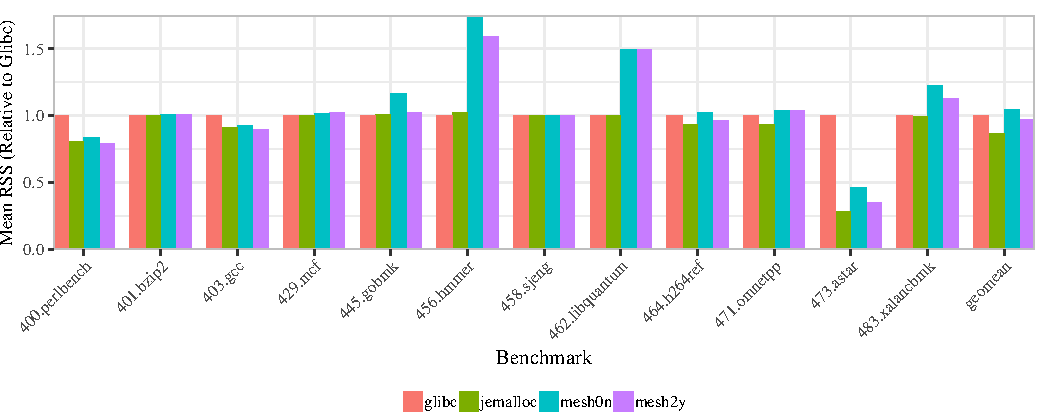
\includegraphics{plots/spec_mem_mean.pdf}
  \caption{\textbf{\Mesh maintains low average memory consumption.}  The SPEC benchmark
    suite does not suffer from serious external fragmentation that
    \Mesh can recover from, but it maintains lower average memory consumption than glibc.
  For \texttt{403.gcc}, \Mesh reduces mean RSS by 15\% (from 220MB to 188MB).}
  \label{fig:spec-mean-rel}
\end{figure*}
\end{comment}

\begin{comment}
\begin{figure*}[!t]
  \centering\small\textbf{~~~~~~~~~SPECint 2006 Absolute Mean RSS}\\[0.3em]
  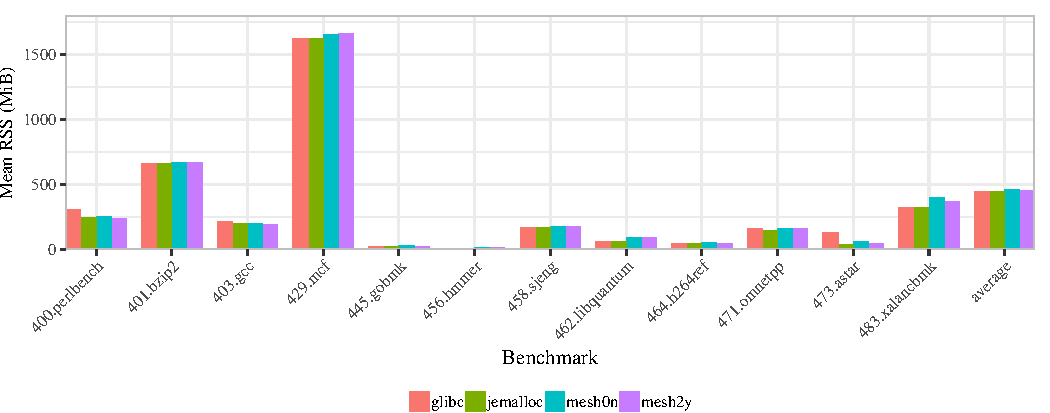
\includegraphics{plots/spec_mem_mean_mb.pdf}
  \caption{\textbf{\Mesh average memory consumption (absolute).}}
  \label{fig:spec-mean}
\end{figure*}
\end{comment}

\begin{comment}
\begin{figure*}[!t]
  \centering\small\textbf{~~~~~~~~~SPECint 2006 Performance}\\[0.3em]
  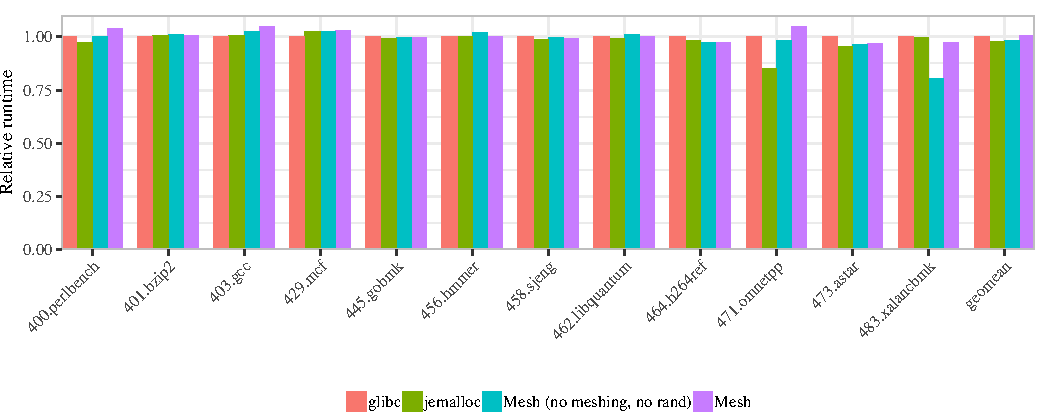
\includegraphics{plots/spec_speed.pdf}
  \caption{\textbf{\Mesh imposes modest runtime overhead.} Performance is
    normalized to glibc. Overall, \Mesh's execution time overhead
    is 15\% higher than glibc's (geometric mean).}
  \label{fig:spec-speed}
\end{figure*}
\end{comment}

\subsection{Memory Savings and Performance Overhead}
\label{sec:evaluation:overallmemory}

We evaluate \Mesh{}'s impact on memory consumption and runtime across
the Firefox web browser, the Redis data structure store, and the
SPECint2006 benchmark suite.

\subsubsection{Firefox}
\label{sec:firefox}

Firefox is an especially challenging application for memory reduction
since it has been the subject of a five year effort to reduce its
memory footprint~\cite{awsy}. To evaluate \Mesh{}'s impact on
Firefox's memory consumption under realistic conditions, we measure
Firefox's RSS while running the Speedometer 2.0 benchmark.
Speedometer was constructed by engineers working on the Google Chrome
and Apple Safari web browsers to simulate the patterns in use on
websites today, stressing a number of browser subsystems like DOM
APIs, layout, CSS resolution and the JavaScript engine.  In Firefox,
most of these subsystems are multi-threaded, even for a single
page~\cite{ff:quantum}.  The benchmark comprises a number of small
``todo'' apps written in a number of different languages and styles,
with a final score computed as the geometric mean of the time taken by
the executed tests.

\begin{figure}[t!]% {.4\linewidth}
  \centering
  \vtop{%
    \centering
    \vskip0pt
    \hbox{%
      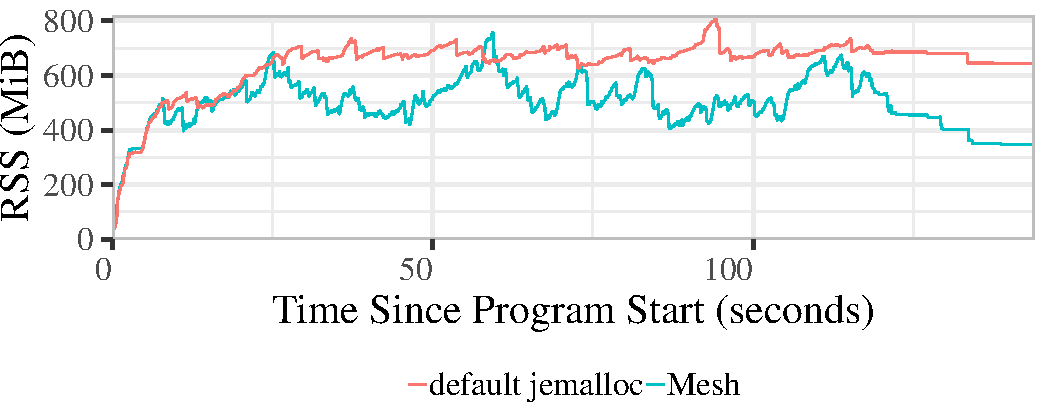
\includegraphics[width=.45\textwidth]{Chapters/mesh/plots/firefox-speedometer.pdf}
    }%
  }
  \caption{\textbf{Firefox:} \Mesh decreases mean heap size by 16\%
    over the course of the Speedometer 2.0 benchmark compared with the
    version of jemalloc bundled with Firefox, with less than a 1\%
    change in the reported Speedometer score (\S\ref{sec:firefox}).
    \label{fig:firefox-heap}}
\end{figure}

We test Firefox in single-process mode (disabling content sandboxing,
which spawns multiple processes) under the \texttt{mstat} tool to
record memory usage over time. Our test opens a tab, loads the
Speedometer page from a local server, waits 2 seconds, and then
automatically executes the test.  We record the reported score
at the end of the benchmark run and calculate average memory
usage recorded by \texttt{mstat}.  We tested both a standard release
build of Firefox, along with a release build that did not bundle
Mozilla's fork of jemalloc (hereafter referred to as
\texttt{mozjemalloc}) and instead directly called \texttt{malloc}-related
functions, with \Mesh included via \texttt{LD\_PRELOAD}.  We report
the average resident set size over the course of the benchmark and a
15 second cooldown period afterward, collecting three runs per
allocator.

\Mesh reduces the memory consumption of Firefox by 16\% compared to
Firefox's bundled jemalloc allocator. \Mesh requires 530 MB ($\sigma =
22.4$ MB) to complete the benchmark, while the Mozilla allocator needs
632 MB ($\sigma = 25.3$ MB). Mesh spent a total of 135 ms meshing over
the course of the benchmark, with a maximum meshing latency of 7.5 ms
and average meshing latency of 0.2 ms.  This result shows that \Mesh
can effectively reduce memory overhead even in widely used and heavily
optimized applications. \Mesh achieves this savings with less than a
1\% reduction in performance (measured as the score reported by
Speedometer).  Hoard and tcmalloc improved Speedometer performance
relative to jemalloc by 5.4 and 6.0\% respectively, while increasing
average heap size by 48.0\% and 8.6\%.

Figure~\ref{fig:firefox-heap} shows memory usage over the course of a
Speedometer benchmark run under \Mesh and the default jemalloc
allocator.  While memory usage under both peaks to similar levels,
Mesh is able to keep heap size consistently lower.


\subsubsection{Redis}
\label{redis-section}


Redis is a widely-used in-memory data structure server.  Redis 4.0
introduced a feature called ``active
defragmentation''~\cite{jemalloc:exposehints,redis:announcement}.
Redis calculates a fragmentation ratio (RSS over sum of active
allocations) once a second.  If this ratio is too high, it triggers a
round of active defragmentation. This involves making a fresh copy of
Redis's internal data structures and freeing the old ones. Active
defragmentation relies on allocator-specific APIs in jemalloc both for
gathering statistics and for its ability to perform allocations that
bypass thread-local caches, increasing the likelihood they will be
contiguous in memory.

\begin{figure}[t!]
  \centering
  \vtop{%
    \centering
    \vskip0pt
    \hbox{%
      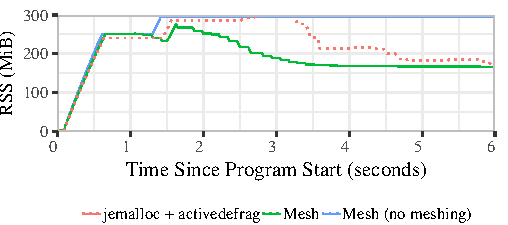
\includegraphics[width=.45\textwidth]{Chapters/mesh/plots/redis-lru.pdf}
    }%
  }
  \caption{\textbf{Redis:} \Mesh automatically achieves significant
    memory savings (39\%), obviating the need for its custom,
    application-specific ``defragmentation'' routine
    (\S\ref{redis-section}).
    \label{fig:redis-results}}
\end{figure}


%This defragmentation
%does not require scanning the heap for pointers because Redis's memory
%primarily consists of a large hash table associating keys with values.


%% A case where active defragmentation is useful is when redis is used as
%% an LRU cache with a maximum heap size set.  If there is a phase shift
%% in the size of objects being added to the cache, redis can suffer from
%% external fragmentation, requiring a significantly larger
%% working-set-size compared to live size of redis allocations.

%% Redis tracks the size of allocations (either through the use of a
%% \texttt{malloc\_usable\_size} API, or by prepending the size to every
%% allocation

We adapt a benchmark from the official Redis test suite to measure how
\Mesh's automatic compaction compares with Redis's active
defragmentation, as well as against the standard glibc allocator. This
benchmark runs for a total of 7.5 seconds, regardless of allocator. It
configures Redis to act as an LRU cache with a maximum of 100 MB of
objects (keys and values).  The test then allocates 700,000 random
keys and values, where the values have a length of 240 bytes.
Finally, the test inserts 170,000 new keys with values of length 492.
Our only change from the original Redis test is to increase the value
sizes in order to place all allocators on a level playing field with
respect to \emph{internal} fragmentation; the chosen values of 240 and
492 bytes ensure that tested allocators use similar size classes for
their allocations. We test \Mesh with Redis in two configurations:
with meshing always on and with meshing disabled, both without any
input or coordination from the redis-server application.

%% Our only change from the original Redis test is to
%% increase the key size in order to place all allocators on a level
%% playing field with respect to \emph{internal} fragmentation; both
%% Hoard and DieHard use power-of-two size classes.

Figure~\ref{fig:redis-results} shows memory usage over time for Redis
under \Mesh, as well as under jemalloc with Redis's
``activedefrag'' enabled, as measured by \texttt{mstat}
(\S\ref{subsec:memory-use}).  The ``activedefrag'' configuration
enables active defragmentation after all objects have been added to
the cache.

Using \Mesh automatically and portably achieves the same heap size
reduction (39\%) as Redis's active defragmentation.  During most of
the 7.5s of this test Redis is idle; Redis only triggers active
defragmentation during idle periods. With \Mesh, insertion takes
1.76s, while with Redis's default of jemalloc, insertion takes 1.72s.
Redis under Hoard and tcmalloc has the same average heap size as Mesh
with meshing disabled (under 2\% difference), and both allocators are
similarly within 2\% of the insertion speed of jemalloc.  \Mesh's
compaction is additionally \textit{significantly} faster than Redis's
active defragmentation. During execution with \Mesh{}, a total of
0.23s are spent meshing (the longest pause is 22 ms), while active
defragmentation accounts for 1.49s ($5.5\times$ slower). This high
latency may explain why Redis disables ``activedefrag'' by default.

%\Mesh's always-on defragmentation comes at a cost, the Redis server
%running with \Mesh is 29\% slower than the default jemalloc (which
%performs no defragmentation).

\subsubsection{SPEC Benchmarks}

%Figure~\ref{fig:spec-mean-rel} presents mean memory consumption (RSS)
%across the SPECint 2006 benchmark suite, normalized to glibc.

%Figure~\ref{fig:spec-mean} presents absolute average memory
%usage.

%% We show that meshing can yield substantial memory savings across a
%% suite of benchmarks and real-world applications, with little runtime
%% overhead. For one of the most allocation-heavy benchmarks in the
%% SPECint suite, \texttt{perlbench}, \Mesh reduces peak RSS by 13\%
%% (across the suite, it decreases average memory consumption by 2.5\%).
%% In longer-lived, memory-intensive applications, \Mesh saves more
%% memory. Replacing Firefox's default allocator with \Mesh reduces
%% average memory consumption in Speedometer 2, a modern browser
%% benchmark, by 11\% (from 651MB to 579MB) with a 6\% reduction in
%% performance.  For the Redis data structure server, \Mesh reduces
%% resident-set size (RSS) by 34\% compared to conventional allocators in
% a fragmentation-heavy workload.


Most of the SPEC benchmarks are not particularly compelling targets
for \Mesh because they have small overall footprints and do not
exercise the memory allocator. For example, while the
\texttt{401.bzip2} benchmark has one of the higher heap size averages
at 665 MB, the difference in both runtime and average heap size
between the fastest + slowest allocators is under 1\%.

Across the entire SPECint 2006 benchmark suite, \Mesh modestly
decreases average memory consumption (geomean: $-2.4$\%) vs. glibc,
while imposing minimal execution time overhead (geomean: 0.7\%).

%% Many Mesh benchmarks are

However, for applications that are both allocation-intensive (many
calls to \texttt{malloc} and \texttt{free}) and which have large footprints,
\Mesh is able to substantially reduce peak memory consumption. The
most allocator-sensitive benchmark is \texttt{400.perlbench}, a Perl
benchmark that performs a number of e-mail related tasks including
spam detection (SpamAssassin). Peak RSS with glibc, jemalloc, and
Hoard is 664 MB, 614 MB, and 732 MB respectively. \Mesh reduces peak
RSS to 564 MB (a 15\% reduction relative to glibc) while increasing
runtime overhead by only 3.9\%.


%\Mesh significantly reduces memory consumption for the
%allocation-heavy SPEC application (\texttt{400.perlbench}: 13\%) while
%imposing a minimal performance penalty.


% As Figure~\ref{fig:spec-speed} shows,
\begin{comment}
though in some cases, its overhead is high. We observe that these
cases correspond with the cases when DieHard also imposes significant
overhead; since both DieHard and \Mesh are randomized memory managers,
we attribute this overhead to degraded locality.
\end{comment}

\subsection{Empirical Value of Randomization}
\label{sec:evaluation:practical}

Randomization is key to \Mesh{}'s analytic guarantees; we evaluate
whether it also can have an observable empirical impact on its ability
to reclaim space. To do this, we test three configurations of \Mesh:
(1) meshing disabled, (2) meshing enabled but randomization disabled,
and (3) \Mesh with both meshing and randomization enabled (the
default).

We tested these configurations with Firefox and Redis, and found no
significant differences when randomization was disabled; we believe
that this is due to the highly irregular (effectively random)
allocation patterns that these applications exhibit. We hypothesized
that a more regular allocation pattern would be more challenging for a
non-randomized baseline. To test this hypothesis, we wrote a synthetic
microbenchmark with a regular allocation pattern in Ruby. Ruby is an
interpreted programming language popular for implementing web
services, including GitHub, AirBnB, and the original version of
Twitter.  Ruby makes heavy use of object-oriented and functional
programming paradigms, making it allocation-intensive.  Ruby is
garbage collected, and while the standard MRI Ruby implementation
(written in C) has a custom GC arena for small objects, large objects
(like strings) are allocated directly with \texttt{malloc}.

Our Ruby microbenchmark repeatedly performs a sequence of string
allocations and deallocations, simulating the effect of accumulating
results from an API and periodically filtering some out. It allocates
a number of strings of a fixed size, then retaining references 25\% of
the strings while dropping references to the rest.  Each iteration the
length of the strings is doubled.  The test requires only a fixed 128
MB to hold the string contents.

\begin{figure}[t!]% {.4\linewidth}
  \centering
  \vtop{%
    \centering
    \vskip0pt
    \hbox{%
      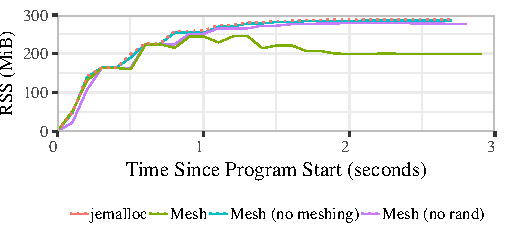
\includegraphics[width=.45\textwidth]{Chapters/mesh/plots/ruby-frag.pdf}
    }%
  }
  \caption{\textbf{Ruby benchmark:} \Mesh is able to decrease mean heap
    size by 18\% compared to \Mesh with randomization disabled and
    non-compacting allocators ($\S$\ref{sec:evaluation:practical}).
    \label{fig:ruby-frag}}
\end{figure}

Figure~\ref{fig:ruby-frag} presents the results of running this
application with the three variants of \Mesh{} and jemalloc; for this
benchmark, jemalloc and glibc are essentially indistinguishable. With
meshing disabled, \Mesh exhibits similar runtime and heap size to
jemalloc. With meshing enabled but randomization disabled, \Mesh
imposes a 4\% runtime overhead and yields only a modest 3\% reduction in
heap size.

Enabling randomization in \Mesh increases the time overhead to 10.7\%
compared to jemalloc, but the use of randomization lets it
significantly reduce the mean heap size over the execution time of the
microbenchmark (a 19\% reduction). The additional runtime overhead is
due to the additional system calls and memory copies induced by the
meshing process.  This result demonstrates that randomization is not
just useful for providing analytical guarantees but can also be
essential for meshing to be effective in practice.

\subsection{Summary of Empirical Results}

For a number of memory-intensive applications, including aggressively
space-optimized applications like Firefox, \Mesh can substantially
reduce memory consumption (by 16\% to 39\%) while imposing a modest
impact on runtime performance (e.g., around 1\% for Firefox and
SPECint 2006). We find that \Mesh{}'s randomization can enable
substantial space reduction in the face of a regular allocation
pattern.

%We find that \Mesh{}'s use of randomization can be
%to reclaim memory

%slightly memory consumption across the SPEC benchmark
%suite and low performance overhead. For two real,
%memory-intensive applications (Firefox and Redis), \Mesh's compaction
%reduces memory consumption significantly with minimal performance
%impact.

%  both reach a steady state where the occupancy of spans containing smaller (240 byte) objects is between 60-65\%, and there are very few spans under half full.


\begin{comment}
  \begin{figure*}[!t]
  \centering\small\textbf{~~~~~~~~~SPECint 2006 Relative Peak RSS}\\[0.3em]
  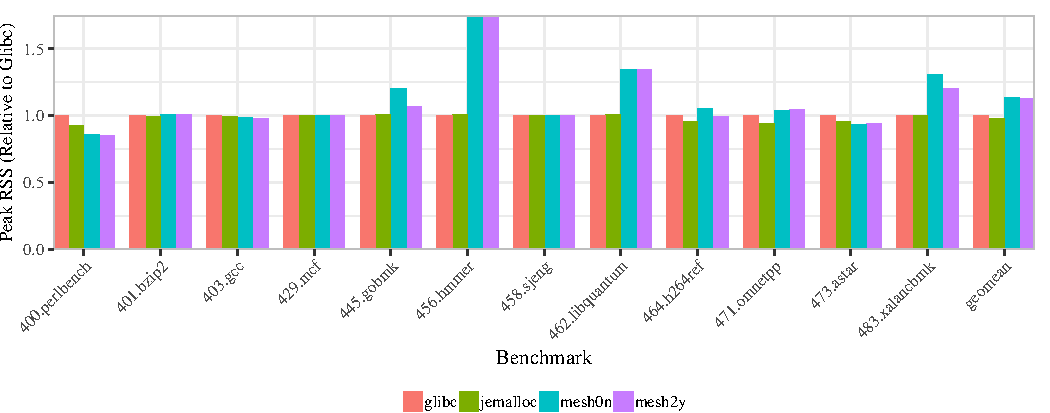
\includegraphics{plots/spec_mem_peak.pdf}
  \caption{\textbf{\Mesh has little impact on peak memory consumption.}
    The meshing algorithm requires additional bookkeeping and
    temporary allocations within the allocator, but these do not
    translate to increased memory usage across SPEC, and sometimes reduce
    it. \Mesh reduces \texttt{400.perlbench}'s peak memory consumption
    by 13.7\% (from 663MB to 575MB).}
  \label{fig:spec-peak-rel}
\end{figure*}
\end{comment}
